
\section{Pre-fit data-MC}
\label{sec:strong:dataMC}
In this section we show the pre-fit agreement between data and the \gls{mc} simulation before the fit in the \gls{cr}
in the distribution of the same kinematic variables as in Section \ref{sec:strong:sigbkg}. 
All the plots show in this section do not include systematic uncertainties and include all the relevant \gls{mc} \glspl{sf}. 
In order to investigate a region of the phase space depleted in signal events the requirement on the number
of b-tagged jets is relaxed to $\nbjet \geq 2$. 

\subsection*{Kinematic reweighting}

The modelling of most kinematic variables related to the energy of the event shows a moderate disagreement 
when compared with data in the 1-lepton channel, while in the agreement is good in the 0-lepton channel. 
This is particularly visible in the distribution of \meff, as shown in Figure \ref{fig:strong:datamc:meff_prerw}.


\begin{figure*}[h]
\centering 
\subfigure[]{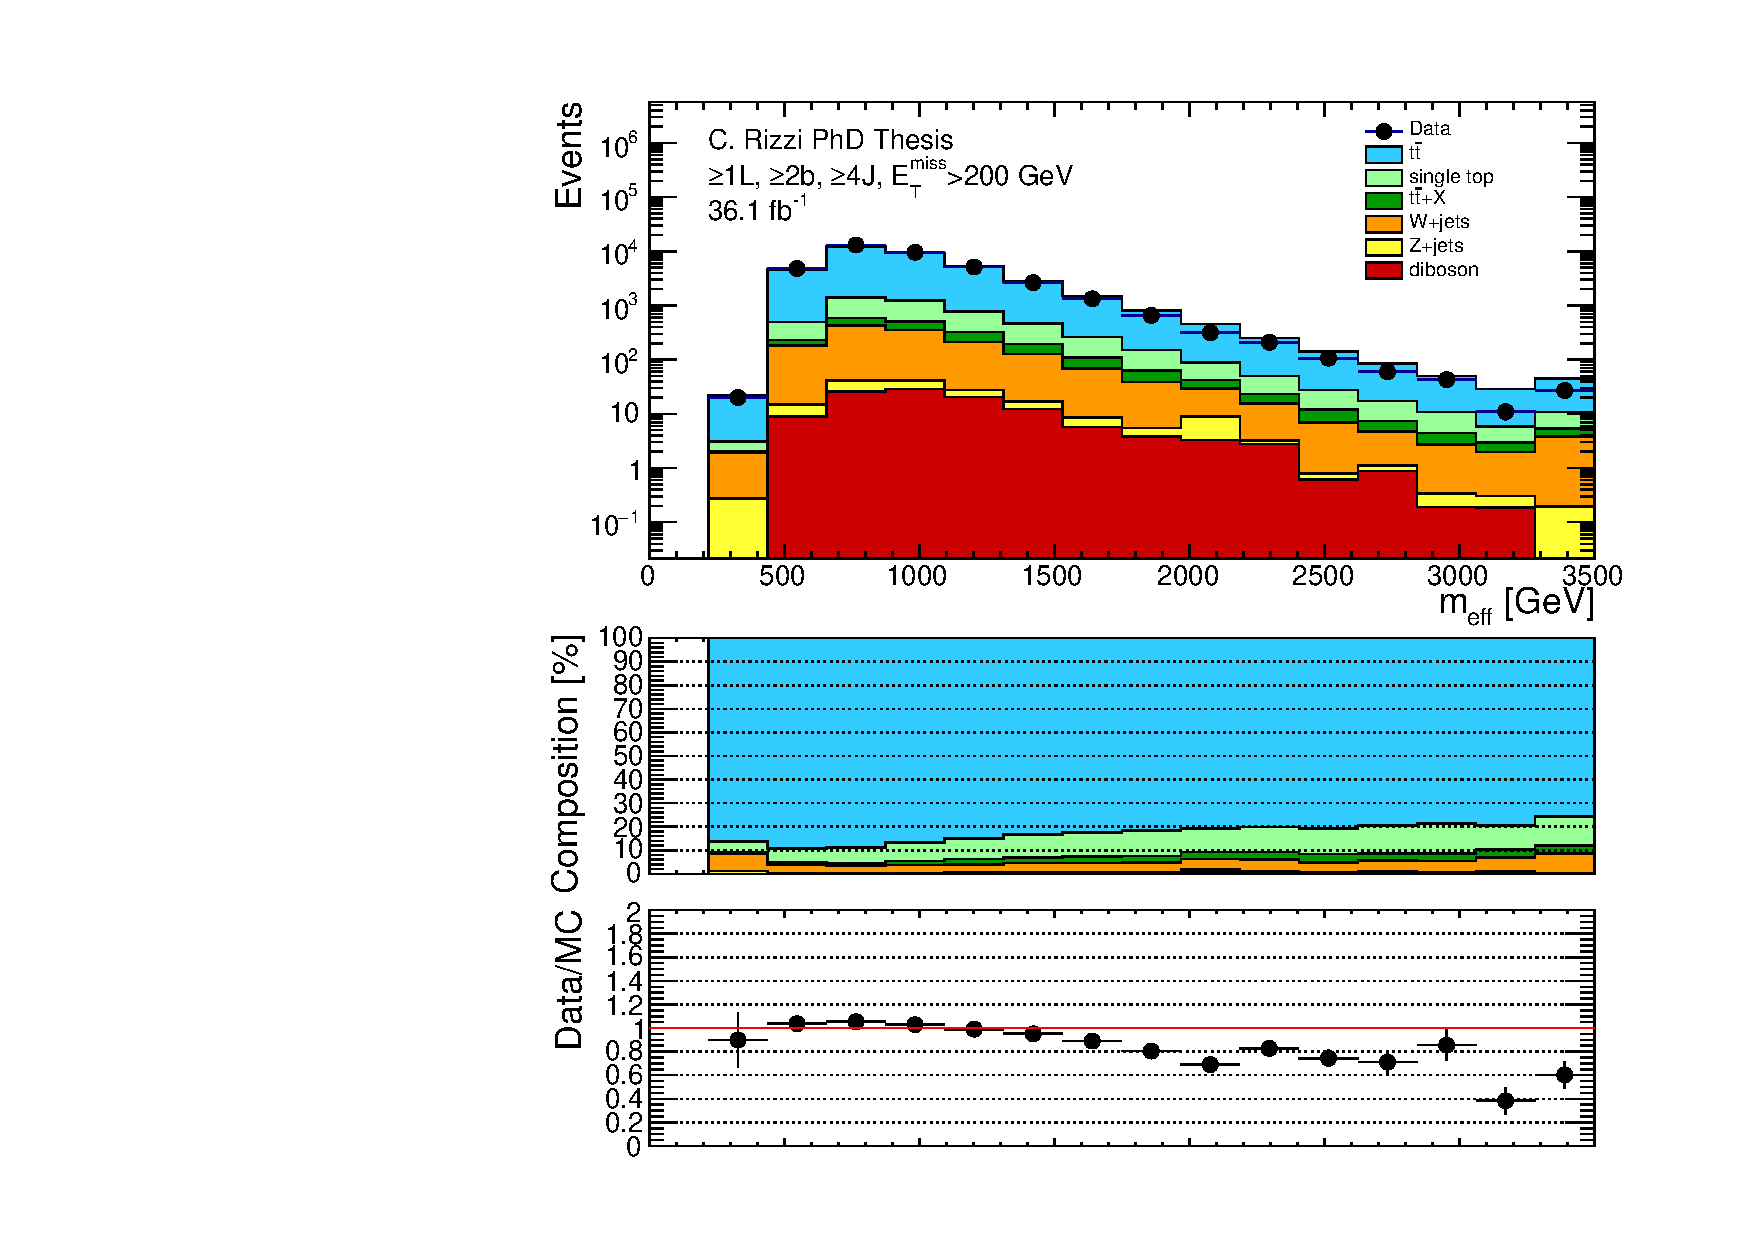
\includegraphics[width=0.49\textwidth]{figures/strong_prod/data_mc/1L_2bin/data_mc_meff_incl.pdf}
\label{fig:strong:datamc:meff_prerw_1L}}
\subfigure[]{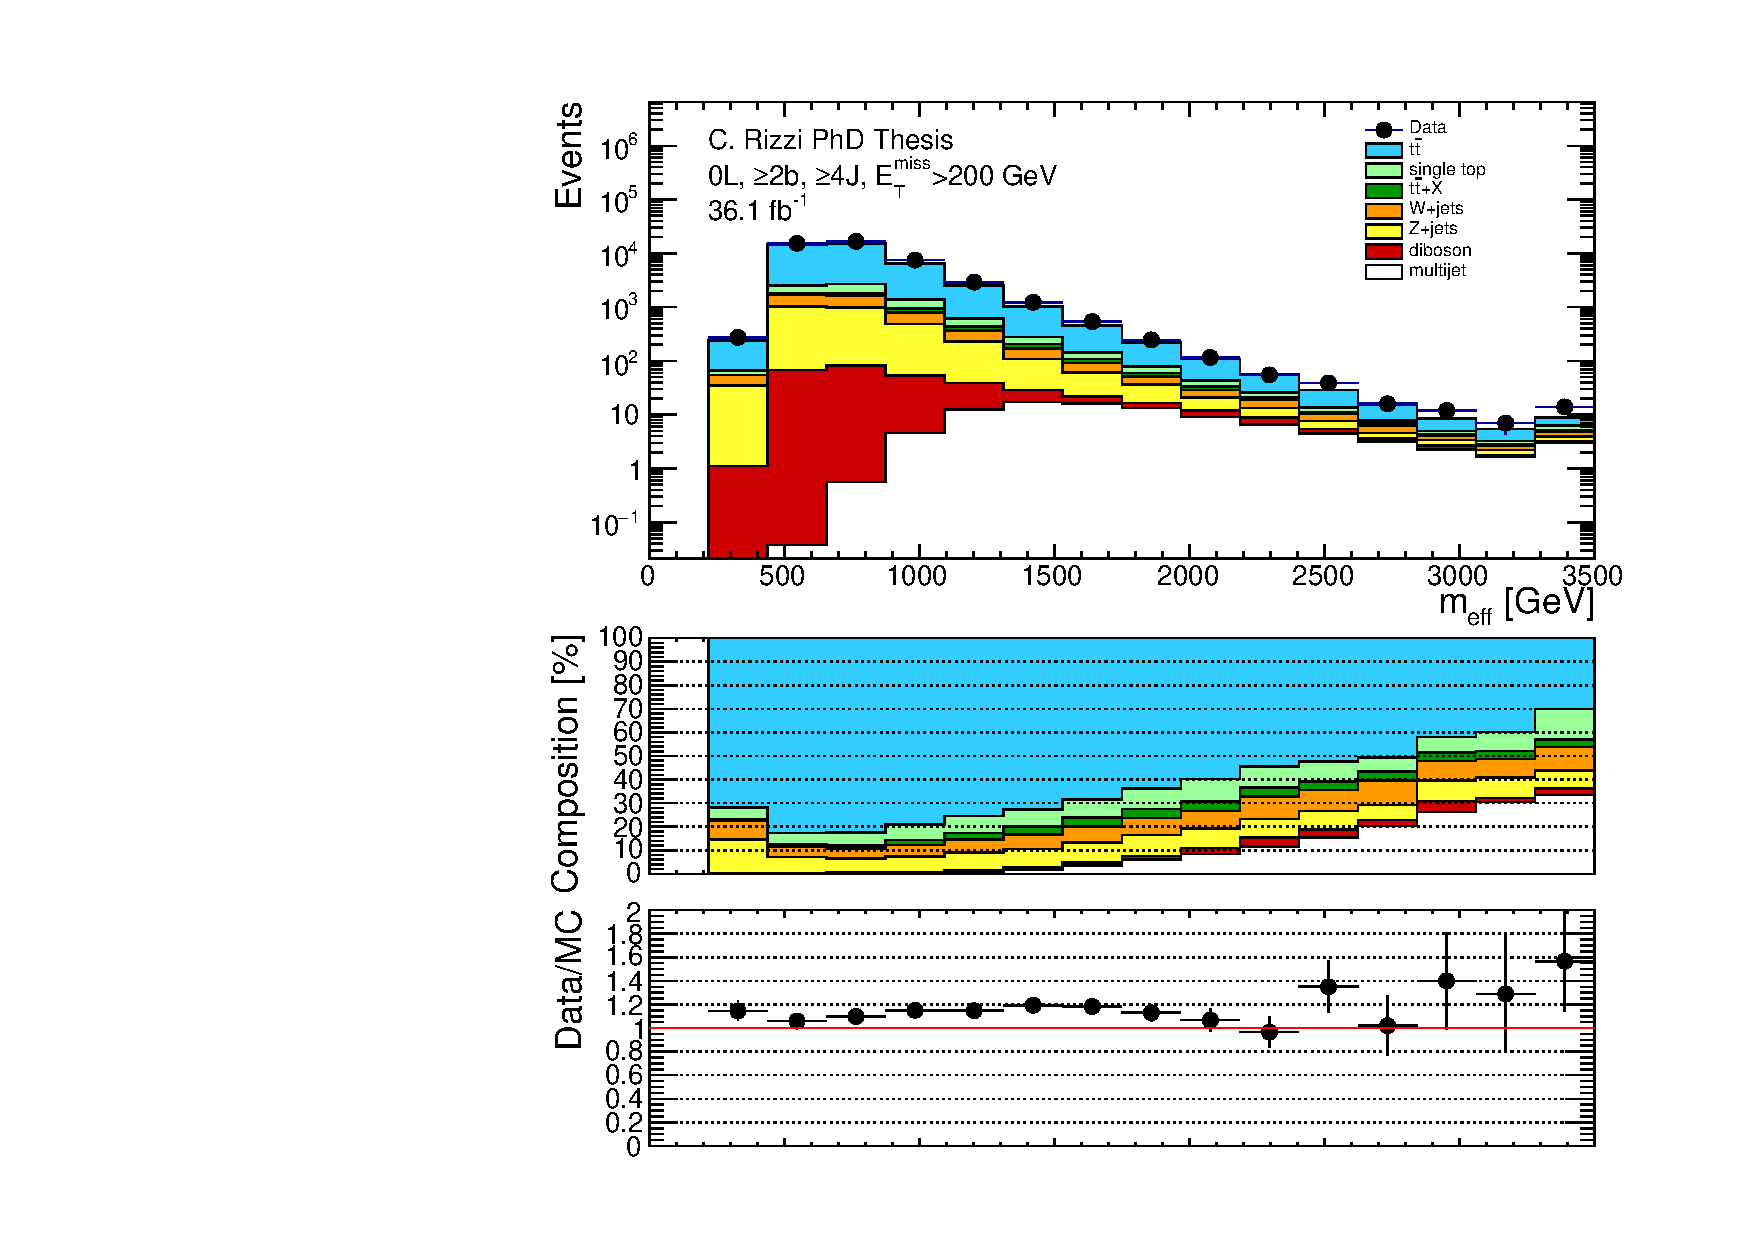
\includegraphics[width=0.49\textwidth]{figures/strong_prod/data_mc/0L_2bin/data_mc_meff_incl.pdf}
\label{fig:strong:datamc:meff_prerw_0L}}
\caption{ \subref{fig:strong:datamc:meff_prerw_1L}
}
\label{fig:strong:datamc:meff_prerw}
\end{figure*}

\subsection*{Data-MC comparison after the reweighting}


